%==============================================================================
%  PART 3 --- ANALYTICAL STUDY (Task 2)
%  Chapters: Descriptive (contracts) | Discourse | Signal-Market Correlation |
%            Cross-Platform | Dashboard
%==============================================================================

\chapter{Descriptive Analysis of Polymarket Contracts}
\label{ch:descriptive}

This chapter characterises the 300 contracts along the dimensions the assignment asks
for --- domain, duration, volume, and volatility --- and then studies how
market-implied probabilities evolve, and how informative they are of the final outcome
at different distances from resolution.

\section{Domain, duration, volume, and volatility}
\Cref{tab:descriptive} summarises the three thematic domains, and reveals that they are
qualitatively different objects despite the equal count.

\begin{table}[H]
\centering
\caption{Descriptive profile of the contracts by thematic domain
(medians; duration IQR in brackets).}
\label{tab:descriptive}
\small
\begin{tabular}{@{}l r r r r r@{}}
\toprule
\textbf{Domain} & \textbf{Contracts} & \textbf{Duration (d)} & \textbf{Volume (USD)} &
\textbf{YES-price vol.} & \textbf{\% YES}\\
\midrule
politics & 100 & 84 \,[28--181] & 25.5\,M & 0.070 & 33\%\\
finance  & 100 & 104 \,[31--134] & 20.8\,M & \textbf{0.114} & 20\%\\
sports   & 100 & \textbf{258} \,[249--272] & \textbf{41.6\,M} & \textbf{0.003} & 4\%\\
\midrule
\textbf{all} & 300 & 154 & 24.9\,M & 0.025 & 19\%\\
\bottomrule
\end{tabular}
\end{table}

\noindent Three patterns stand out (\Cref{fig:durvol,fig:volat}):
\begin{itemize}
  \item \textbf{Sports contracts are long-lived, high-volume long-shots.} They run for
  a whole season (median 258 days), attract the largest median volume, yet have the
  \emph{lowest} price volatility ($0.003$) and resolve \textsc{No} 96\% of the time ---
  they are mostly ``will team $X$ win the league?'' markets that sit near a stable, low
  probability for months and then resolve against the field.
  \item \textbf{Finance contracts are the most volatile} ($0.114$): crypto price-level
  bets (``Bitcoin above \$$X$'') swing as the underlying asset moves.
  \item \textbf{Politics contracts are the shortest and most balanced} in outcome
  (33\% \textsc{Yes}), consistent with sharp, event-driven questions.
\end{itemize}

\begin{figure}[H]
\centering
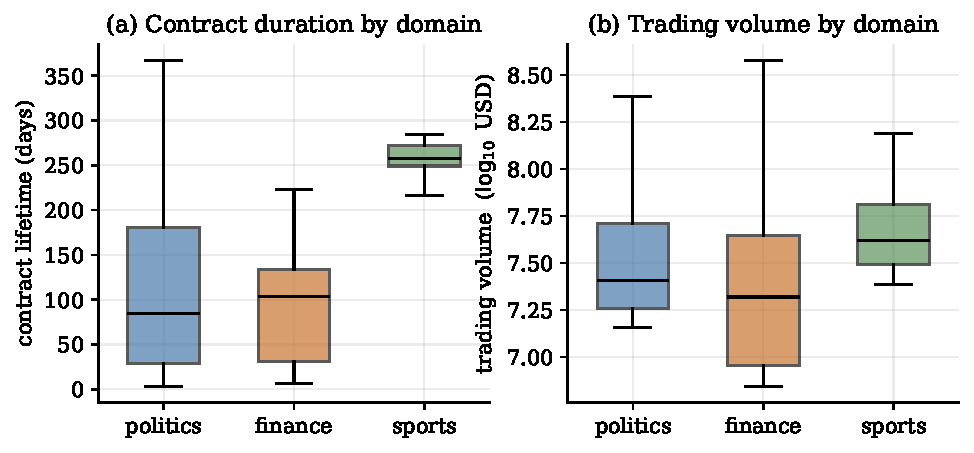
\includegraphics[width=\linewidth]{fig_duration_volume.pdf}
\caption{Contract lifetime (a) and trading volume (b) by domain. Sports contracts are
markedly longer-lived; volumes are large across the board (note the $\log_{10}$ scale).}
\label{fig:durvol}
\end{figure}

\begin{figure}[H]
\centering
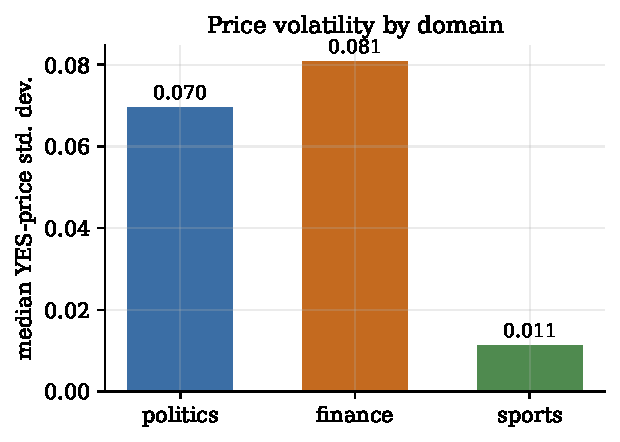
\includegraphics[width=0.56\linewidth]{fig_price_volatility.pdf}
\caption{Median volatility of the \textsc{Yes} price by domain. Finance is an order of
magnitude more volatile than sports.}
\label{fig:volat}
\end{figure}

\section{Are prices informative of the outcome?}
\label{sec:informative}
The central descriptive question is whether the market price is informative of the
final outcome, and how that informativeness depends on the distance to resolution. We
take, for each contract, the latest \textsc{Yes} price at least $h$ days before close,
treat it as a probabilistic forecast $\hat{p}=\Pr(\textsc{Yes})$, and score it against
the realised outcome with AUC and the Brier score
$\frac{1}{N}\sum_i (\hat{p}_i - y_i)^2$~\cite{brier1950verification}.
\Cref{fig:informative} shows the result.

\begin{figure}[H]
\centering
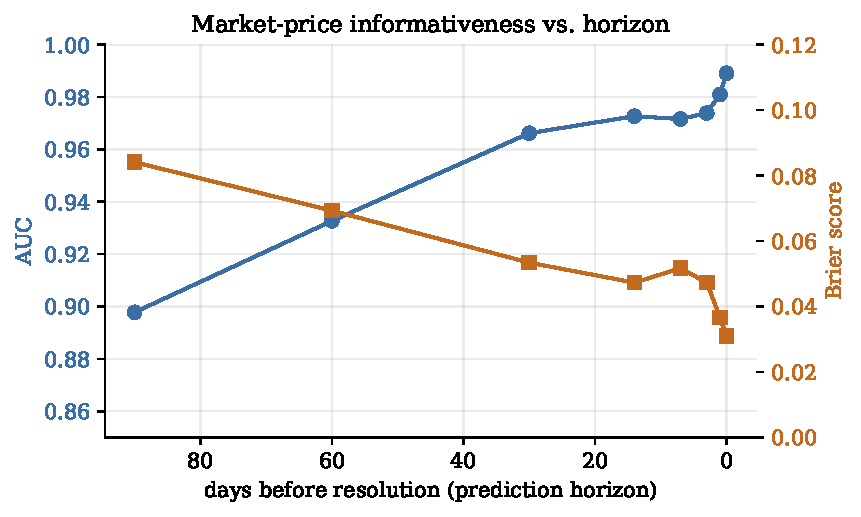
\includegraphics[width=0.72\linewidth]{fig_price_informativeness.pdf}
\caption{Market-price informativeness as a function of the prediction horizon (the
$x$-axis runs from 90 days before resolution, left, to the close, right). AUC rises
monotonically from $0.90$ to $0.99$ and the Brier score falls from $0.084$ to $0.031$
as resolution approaches.}
\label{fig:informative}
\end{figure}

\noindent The market is already a \emph{strong} forecaster three months out (AUC
$0.90$) and becomes near-perfect at the close (AUC $0.99$, Brier $0.031$). This is the
textbook behaviour of an efficient market resolving uncertainty over
time~\cite{wolfers2004prediction}, and it has a decisive consequence for the rest of
the report: \textbf{the bar any social signal must clear --- adding value on top of a
price that is already this informative --- is very high}. We return to this in
\Cref{ch:prediction}.

\begin{takeaway}
The market price alone separates \textsc{Yes} from \textsc{No} contracts with
AUC~$0.90$ three months before resolution and AUC~$0.99$ at the close. Informativeness
grows monotonically as the event nears.
\end{takeaway}


%==============================================================================
\chapter{Social-Media Discourse Analysis}
\label{ch:discourse}

We now characterise the discourse: its volume and timing, its sentiment, the entities
and topics that dominate it, and how these differ across platforms and domains
(Task~2.2).

\section{Volume, timing, and sources}
The corpus spans a decade of channel history but is concentrated in recent years, with
the analysis focused on the post-2024 window in which the studied contracts are active
(\Cref{fig:volume}). It is overwhelmingly a \textbf{Telegram} corpus
(98.6\%); Reddit contributes 16{,}254 posts (1.2\%) and X/Twitter a further 2{,}822
(0.2\%), a small but real third platform whose scale is capped by its anti-automation
defences (\Cref{sec:scope}). Volume is concentrated in a handful of large channels
(\Cref{fig:channels}): crypto exchanges and news aggregators (\code{CryptoComOfficial},
\code{cointelegraph}), macro/markets feeds (\code{zerohedge}, \code{FinancialJuice},
\code{WalterBloomberg}), and geopolitics/OSINT channels (\code{nexta\_live},
\code{ClashReport}, \code{intelslava}, \code{rybar}). This channel mix is the single
most important fact about the corpus: \textbf{it is a crypto/macro/geopolitics corpus,
with essentially no sports coverage} --- a mismatch we quantify in
\Cref{ch:crossplatform}.

\begin{figure}[H]
\centering
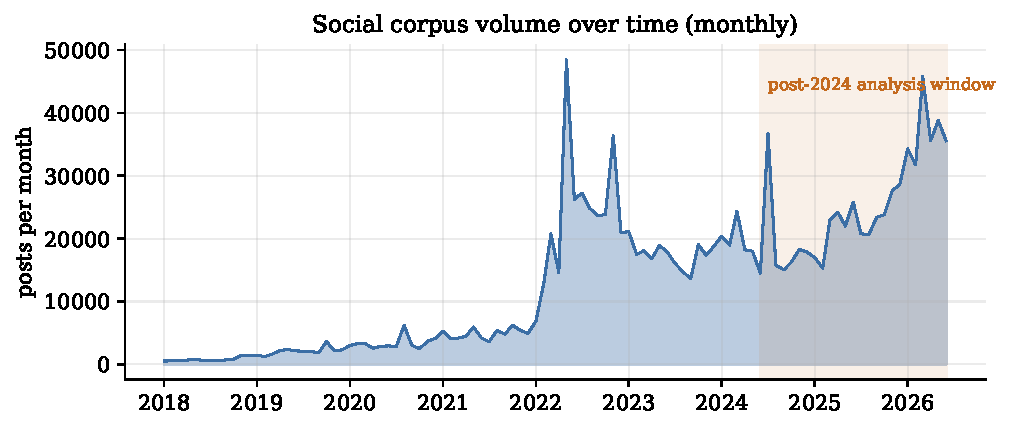
\includegraphics[width=\linewidth]{fig_social_volume.pdf}
\caption{Monthly volume of the social corpus. Activity accelerates through 2024--2026;
the shaded region marks the analysis window in which the studied contracts are live.}
\label{fig:volume}
\end{figure}

\begin{figure}[H]
\centering
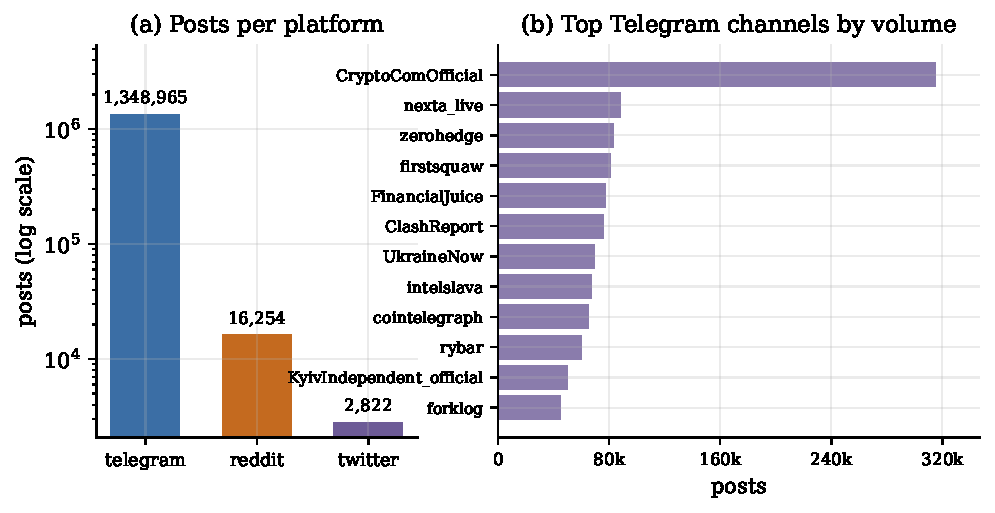
\includegraphics[width=\linewidth]{fig_corpus_platform_channels.pdf}
\caption{(a) Posts per platform (log scale): Telegram dominates. (b) The largest
Telegram channels are crypto, macro, and geopolitics sources.}
\label{fig:channels}
\end{figure}

\section{Sentiment}
Sentiment, computed with VADER (\Cref{ch:nlp}), is close to balanced but slightly
positive on aggregate (mean compound $+0.006$): \textbf{48\% neutral, 28\% positive,
24\% negative} (\Cref{fig:sentiment}). The neutral mass is expected for a corpus heavy
in news-wire and OSINT reporting (``\textsc{Breaking}: \dots''), whose register is
factual. The platform breakdown is similar on Telegram and Reddit, so sentiment does
not, by itself, distinguish the two sources.

\begin{figure}[H]
\centering
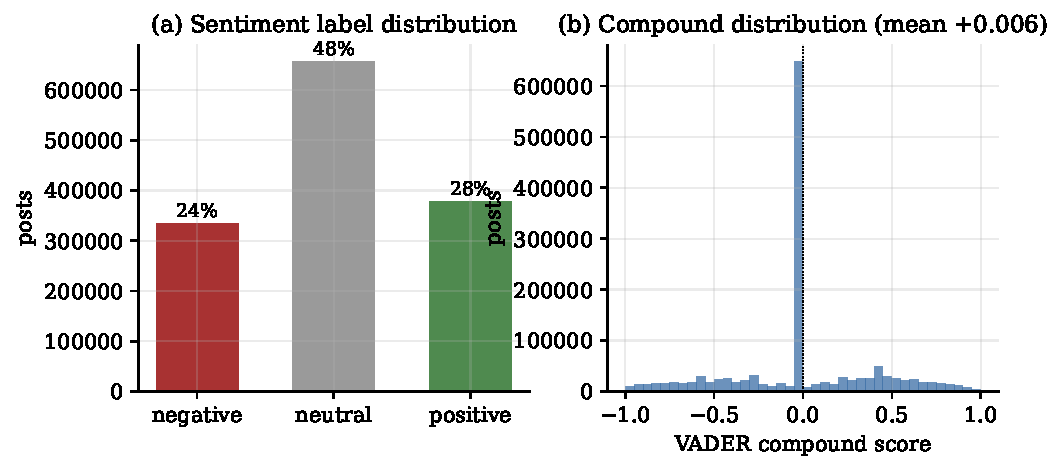
\includegraphics[width=\linewidth]{fig_sentiment.pdf}
\caption{(a) Sentiment-label distribution over 1{,}368{,}041 enriched posts. (b) The VADER
compound score is centred near zero with a slight positive tilt.}
\label{fig:sentiment}
\end{figure}

\section{Named entities}
The most frequent entities (\Cref{fig:entities}) trace the corpus's preoccupations:
\emph{Trump}, the \emph{US}, \emph{Ukraine}, \emph{Iran}, \emph{Russia}, \emph{Israel},
\emph{Gaza}, the \emph{Fed}, \emph{China}, and \emph{Bitcoin}. The list confirms a
politics, geopolitics, macro, and crypto corpus, and the near-total absence of sports
entities. It also exposes an honest limitation of the heuristic NER backend: a few
high-frequency ``entities'' are in fact channel handles or news boilerplate (e.g.\
broadcast-footer tokens, app names such as \emph{WhatsApp} and \emph{Viber}, and markers
like \emph{Breaking} or \emph{Just In}). We filter the most obvious of these from
\Cref{fig:entities}; a
production system would use the spaCy backend (available but not used at scale here) and
a stop-entity list. The artefact does not affect the predictive results, which depend on
stance, not on raw entity counts.

\begin{figure}[H]
\centering
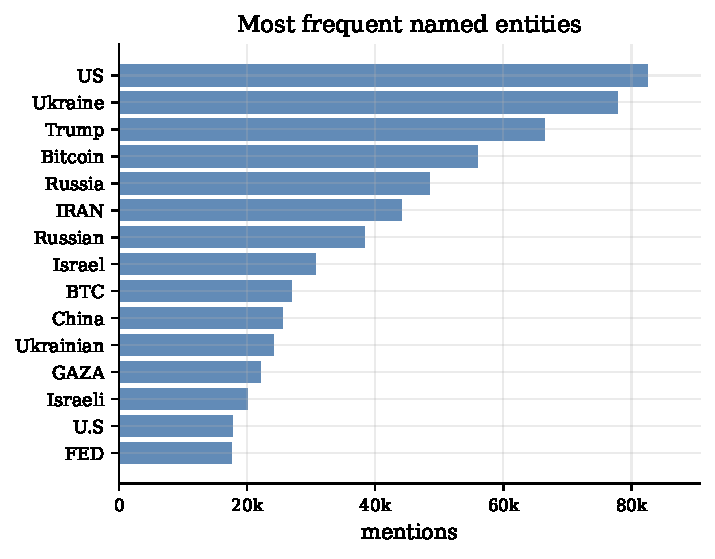
\includegraphics[width=0.66\linewidth]{fig_entities.pdf}
\caption{Most frequent named entities (obvious channel/app/boilerplate tokens removed).
The corpus is dominated by geopolitics, macro, and crypto references.}
\label{fig:entities}
\end{figure}

\section{Topics}
Latent Dirichlet Allocation over the linked posts yields ten coherent topics
(\Cref{fig:topics,tab:topics}). They partition cleanly into \emph{geopolitics}
(Iran--Israel strikes, Iran nuclear talks, Trump and Ukraine, the Iranian regime),
\emph{macro} (Fed, rates, inflation), and \emph{crypto} (Bitcoin, Ethereum, and
trading groups). No topic is about sports. The topic structure thus mirrors the
entity and channel analyses: three things the corpus talks about a great deal, and one
of the three required domains it barely mentions.

\begin{figure}[H]
\centering
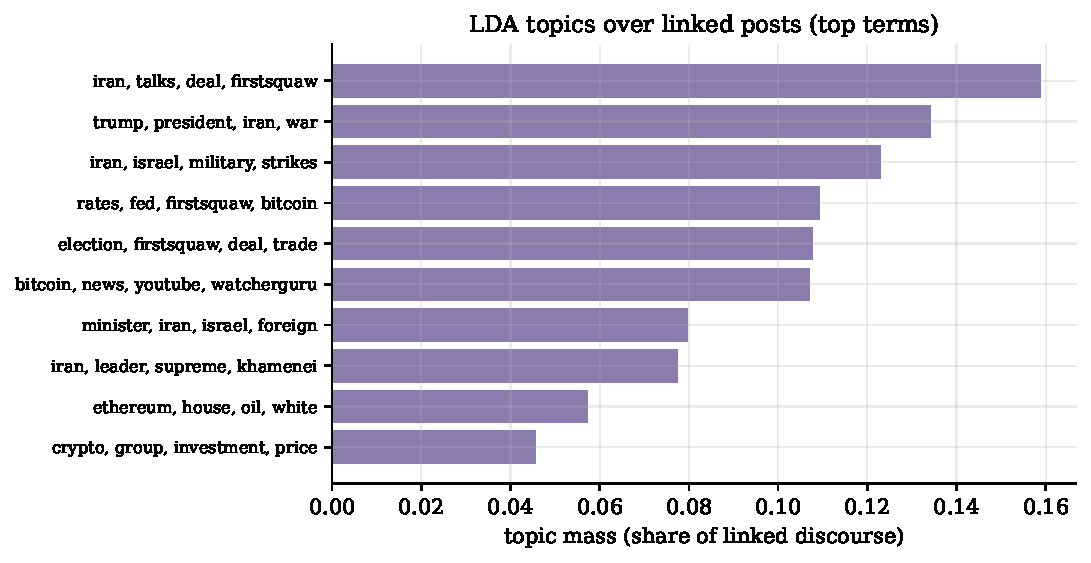
\includegraphics[width=0.74\linewidth]{fig_topics.pdf}
\caption{LDA topic mass over the linked discourse. Geopolitics, macro, and crypto
topics dominate; sports is absent.}
\label{fig:topics}
\end{figure}

\begin{table}[H]
\centering
\caption{The ten LDA topics over linked posts, by mass, with their leading terms.}
\label{tab:topics}
\small
\begin{tabularx}{\linewidth}{@{}r l X@{}}
\toprule
\textbf{Mass} & \textbf{Theme} & \textbf{Top terms}\\
\midrule
0.159 & Iran nuclear talks & iran, talks, deal, trump, russia, nuclear, ukraine\\
0.134 & Trump / war / Ukraine & trump, president, iran, war, ukraine, russia, ceasefire\\
0.123 & Iran--Israel strikes & iran, israel, military, strikes, iranian, missile, regime\\
0.109 & Fed / rates & rates, fed, inflation, policy, rate, hold, cut\\
0.108 & Elections / trade & election, deal, trade, rates, fed, president, japan\\
0.107 & Bitcoin / crypto news & bitcoin, news, btc, crypto, ethereum, saylor, bank\\
0.080 & Diplomacy / ministers & minister, iran, israel, foreign, prime, rubio, security\\
0.077 & Iran supreme leader & iran, leader, supreme, khamenei, iranian, killed\\
0.057 & Ethereum / oil / WH & ethereum, house, oil, white, buterin, vitalik\\
0.046 & Crypto trading groups & crypto, group, investment, price, sell, buy, discussion\\
\bottomrule
\end{tabularx}
\end{table}


%==============================================================================
\chapter{Signal--Market Correlation}
\label{ch:correlation}

This chapter studies the temporal relationship between the social signal and the market
price (Task~2.3): does social activity precede, coincide with, or follow price moves,
and is the direction of social stance aligned with the direction of price change?

\section{Constructing the social signal}
\label{sec:spi-signal}
To compare social discourse against price on the same axis, we condense the accepted,
directional evidence into a per-day social estimate of $\Pr(\textsc{Yes})$. Let
$w^{+}_t$ and $w^{-}_t$ be the day-$t$ \textsc{Yes}/\textsc{No} evidence weights, where
each stance contributes $\text{confidence}\times(1+\log(1+\text{engagement}))$, capped
at $4.0$ per post and at $3.0$ per source per market-day so that no single author or
channel dominates a market-day (source diversity), and the
daily totals are EWMA-smoothed with a 3-day half-life. The social signal and its
strength are then
\begin{equation}
s_t \;=\; \frac{w^{+}_t + \tfrac{\kappa}{2}}{w^{+}_t + w^{-}_t + \kappa},
\qquad
\sigma_t \;=\; \frac{w^{+}_t + w^{-}_t}{w^{+}_t + w^{-}_t + \kappa}\;\in[0,1),
\label{eq:signal}
\end{equation}
a Laplace-smoothed estimate anchored at $0.5$ with pseudo-count $\kappa=1.5$
(implemented as a per-side $\alpha=0.75$): on thin-evidence days $\sigma_t\!\approx\!0$
and $s_t\!\approx\!0.5$, so the signal does not spike on noise. We treat the social line
as meaningful only where $\sigma_t$ is well above zero.

\section{Do social spikes lead, coincide with, or follow price moves?}
We answer this quantitatively. On days with meaningful evidence ($\sigma_t>0.2$;
$1{,}848$ contract-days over $66$ contracts), the pooled Pearson correlation between
$s_t$ and the market probability is only $\mathbf{0.05}$, and the median per-contract
correlation is $0.09$ (\Cref{fig:leadlag}b) --- weak and scattered around zero. To test
\emph{direction}, we cross-correlate daily \emph{changes}, $\Delta s_t$ against
$\Delta p_{t+k}$, for lags $k\in[-7,7]$ pooled over the well-covered contracts
(\Cref{fig:leadlag}a): a positive lag $k$ means the price moves \emph{after} the social
signal, i.e.\ social would be \emph{leading}. The profile is essentially flat --- every
lag stays within $|r|<0.04$ --- and the only mild peak sits at lag $0$ (coincident), with
\textbf{no positive-lead peak}. There is therefore no horizon at which social changes
systematically precede price changes: the little structure that exists is coincident at
best, consistent with discourse \emph{reacting} to, rather than anticipating, the events
the market prices.

\begin{figure}[H]
\centering
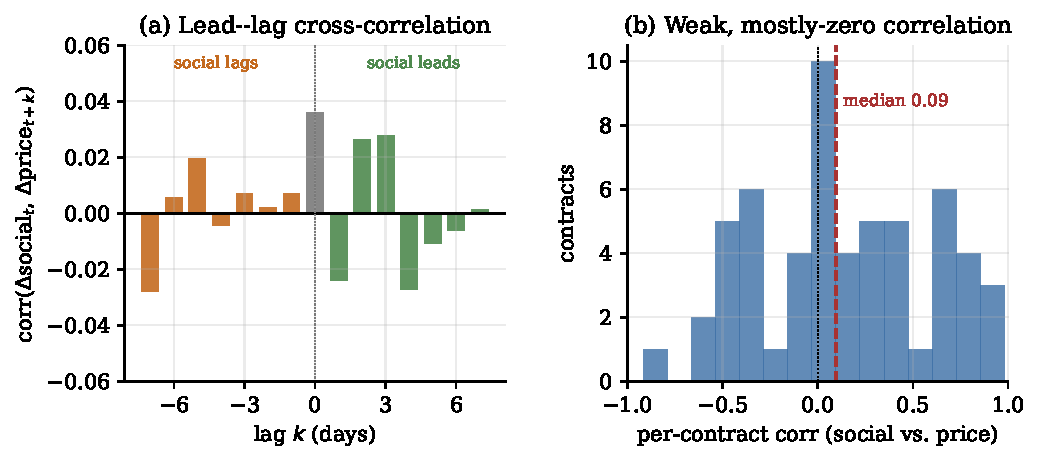
\includegraphics[width=\linewidth]{fig_leadlag.pdf}
\caption{Social signal versus price, quantitatively. (a)~Lead--lag cross-correlation of
daily changes: a positive lag ($k>0$) would mean social \emph{leads} the price, yet every
lag stays within $|r|<0.04$ and the only mild peak is at lag $0$ (coincident) --- there is
no positive-lead peak. (b)~Distribution of per-contract social--price correlations: weak
and centred near zero (median $0.09$). Together they show the social signal neither leads
nor meaningfully tracks the market price.}
\label{fig:leadlag}
\end{figure}

\section{Is the direction of stance aligned with the outcome?}
Aggregating stance into a per-contract direction (\Cref{eq:signal} at the final
pre-close cut), the directional agreement between the social signal and the realised
outcome is only $\mathbf{0.21}$ --- worse than a coin flip --- and the correlation
between the aggregate stance balance and the outcome is $-0.015$ (essentially zero). The
reason is the optimism mismatch already visible in \Cref{fig:stance}: among the
72 contracts on which social pressure points \textsc{Yes}, only 14 actually resolved
\textsc{Yes} (\Cref{fig:hype}). Social discourse is systematically biased towards the
exciting \textsc{Yes} outcome, while the contracts overwhelmingly resolve \textsc{No}.

\begin{figure}[H]
\centering
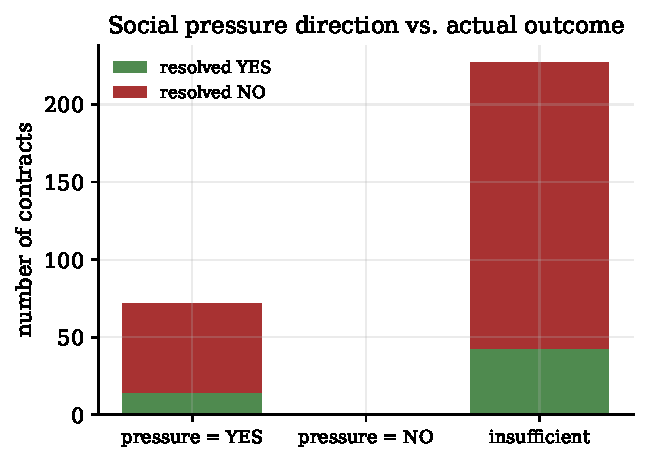
\includegraphics[width=0.56\linewidth]{fig_hype_mismatch.pdf}
\caption{Social-pressure direction versus actual outcome. Where social pressure says
\textsc{Yes} (72 contracts), the market still resolves \textsc{No} 58 times; the social
direction is anti-correlated with reality.}
\label{fig:hype}
\end{figure}

\begin{takeaway}
Social activity neither leads nor strongly coincides with price (pooled correlation
$0.05$, flat lead--lag profile), and its \emph{direction} is anti-aligned with outcomes
(agreement $0.21$). The discourse is reactive and optimism-biased.
\end{takeaway}


%==============================================================================
\chapter{Cross-Platform Comparison}
\label{ch:crossplatform}

Task~2.4 asks three concrete questions: do the platforms carry \emph{complementary} or
\emph{redundant} signals; are there contracts for which one platform is substantially
more informative than the others; and what distinguishes those cases. This chapter
answers each over all three collected platforms (Telegram, Reddit, and X/Twitter),
with Telegram supplying the overwhelming majority of posts (\Cref{sec:scope}). The
cross-platform layer reads from \code{cross\_platform\_comparison.parquet} (one row
per contract that carries social discourse) and its per-domain roll-up
\code{cross\_platform\_summary.parquet}.

\section{How many platforms cover each contract?}
\label{sec:xplat-coverage}
Of the 300 contracts, \textbf{232 carry at least one linked social post}, and
\textbf{181 of those are multi-platform} --- discussed on at least two of Telegram,
Reddit, and X/Twitter within the analysis window, with \textbf{114 carrying all three}.
\Cref{tab:xplat} breaks the 232 down by domain, and \Cref{fig:xplat} visualises it.

\begin{table}[H]
\centering
\caption[Per-domain platform coverage]{Platform coverage by domain over the 232 contracts
that carry social discourse. \emph{Single} = one platform present;
\emph{multi} = at least two platforms present; \emph{compl.} = contracts the
cross-platform analysis flags as genuinely \emph{complementary} (a minority platform
contributes non-trivially rather than echoing the majority).}
\label{tab:xplat}
\small
\begin{tabular}{@{}l r r r r@{}}
\toprule
\textbf{Domain} & \textbf{With social} & \textbf{Single-platform} & \textbf{Multi-platform} & \textbf{Complementary}\\
\midrule
politics & 85  & 21 & 64  & 1\\
finance  & 58  & 10 & 48  & 0\\
sports   & 89  & 20 & 69  & \textbf{28}\\
\midrule
\textbf{total} & \textbf{232} & 51 & 181 & 29\\
\bottomrule
\end{tabular}
\end{table}

\begin{figure}[H]
\centering
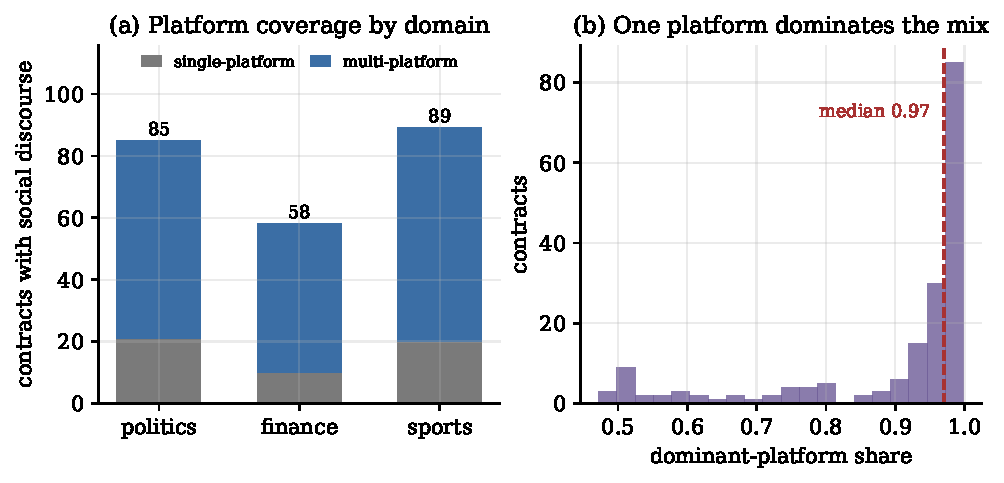
\includegraphics[width=\linewidth]{fig_cross_platform.pdf}
\caption{Cross-platform coverage. (a)~Single- vs multi-platform contracts by domain:
most covered contracts appear on both platforms. (b)~Distribution of the
\emph{dominant-platform share} over multi-platform contracts --- Telegram supplies the
overwhelming majority of posts even when Reddit is also present, so the two signals are
mostly \textbf{redundant rather than complementary}.}
\label{fig:xplat}
\end{figure}

\section{Redundant or complementary?}
On the 181 multi-platform contracts the \emph{dominant platform} (Telegram in almost
every case) accounts for a median share of ${\sim}\mathbf{0.97}$ of the posts: when
several platforms speak about a contract, they say the same thing and Telegram says far
more of it. By the standard meaning of the question, the signals are therefore
\textbf{redundant, not complementary} --- adding Reddit or X to Telegram rarely changes
the per-contract social estimate. The lone exception is \textbf{sports}: 28 sports
contracts are flagged complementary, precisely because Telegram barely covers sports
(\Cref{sec:xplat-mismatch}), so what little signal exists there comes disproportionately
from Reddit. This is the one corner of the dataset where a second platform measurably
adds coverage.

\section{Where is one platform substantially more informative?}
The per-contract view identifies the cases the assignment asks for. For
\emph{geopolitics and macro} contracts --- US--Iran, Russia--Ukraine, the Fed --- Telegram
is overwhelmingly the more informative platform, contributing thousands of posts where
Reddit contributes tens. For the handful of \emph{sports} contracts that are covered at
all, Reddit is relatively (though still thinly) the more informative source. No contract
in the snapshot is substantially better covered by Reddit than Telegram in absolute
terms; that asymmetry is a property of the collected channel mix, and the cross-platform
table is the artefact that would surface the reverse cases under a broader collection.

\section{A genuine three-platform comparison}
Because every platform normalises to the same \code{SocialPostRecord} and the
cross-platform analysis keys only on \code{platform}, all three sources enter
\Cref{tab:xplat,fig:xplat} uniformly: \textbf{114 of the 232 covered contracts carry
posts from all three platforms}. X/Twitter's contribution is small in volume
(\Cref{sec:scope}), so Telegram still dominates the per-contract mix, but the comparison
is genuinely three-platform rather than a two-platform result with a placeholder column.
Broadening the X or Reddit pass would repopulate this chapter with no code change ---
re-running \code{polysignal analytics run} followed by the figure regeneration is all
that is required.

\section{The channel--market mismatch}
\label{sec:xplat-mismatch}
The more consequential cross-cutting comparison is not between platforms but between
the \emph{topics} the channels discuss and the \emph{domains} of the contracts.
\Cref{tab:mismatch} lays the mismatch bare: politics contracts absorb 81\% of all
accepted evidence, finance most of the rest, and \textbf{sports almost none} (211 links
across 100 contracts). The channels are crypto/macro/geopolitics sources; they simply do
not talk about who will win the Premier League.

\begin{table}[H]
\centering
\caption{Accepted evidence by domain, against the equal contract counts. Social evidence
is concentrated where the channels' topics lie, not where the contracts are.}
\label{tab:mismatch}
\small
\begin{tabular}{@{}l r r r@{}}
\toprule
\textbf{Domain} & \textbf{Contracts} & \textbf{Accepted links} & \textbf{Share of evidence}\\
\midrule
politics & 100 & 30{,}387 & 80.9\%\\
finance  & 100 & 6{,}964  & 18.5\%\\
sports   & 100 & 211      & 0.6\%\\
\midrule
\textbf{total} & 300 & 37{,}562 & 100\%\\
\bottomrule
\end{tabular}
\end{table}

\noindent The contracts for which social discourse is by far the most informative are
therefore the \emph{geopolitics} ones --- US--Iran, Russia--Ukraine, Israel--Iran ---
which attract thousands of accepted links each, while crypto price-level and Fed-rate
contracts attract hundreds and sports contracts attract a handful. This is the key
qualitative finding of the cross-cutting analysis, and it directly explains the
predictive results of Part~IV: the social signal is dense and usable for one slice of
the market and absent for another.


%==============================================================================
\chapter{Interactive Dashboard}
\label{ch:dashboard}

All results are exposed through a custom interactive \textbf{React}~\cite{react}
single-page application (designed and built with Claude's design tooling, \emph{not} the
suggested Streamlit~\cite{streamlit2023} default, to obtain a more polished and
customisable interface). It is served on a single local origin by a small, zero-dependency
Python API (\code{scripts/serve\_app.py}, launched by \code{run\_app.cmd}) that materialises
the exact persisted artefacts behind this report into the \code{window.PS\_DATA} contract:
the app needs \emph{no internet, no CORS, and no build step}, never recomputes features,
retrains models, or calls an external service, so a live demo is deterministic and fast.
The application is the deliverable shown live during the oral discussion.

\section{Views}
The app is organised as two linked views plus a persistent customisation panel
(\Cref{tab:dashboard}). It opens on the \emph{Market Universe}; selecting any contract
drills into the \emph{Market Detail}.

\begin{table}[H]
\centering
\caption{The React dashboard: views, the panels they contain, and the Task-2 requirement
each satisfies.}
\label{tab:dashboard}
\small
\begin{tabularx}{\linewidth}{@{}l X@{}}
\toprule
\textbf{View / panel} & \textbf{What it shows}\\
\midrule
\textbf{Market Universe} & browse all 300 contracts as a card grid; filter by \emph{domain} (macro, politics, crypto, AI, sports, culture) and \emph{status} (active, closing, resolved); each card sparklines price vs.\ social signal\\
\textbf{Market Detail} & opens on the per-contract \emph{dual-line chart}: market $\Pr(\textsc{Yes})$ vs.\ the smoothed social signal (\Cref{eq:signal}), with event markers\\
\quad Social panel        & post volume, sentiment split, and the stance distribution for the contract\\
\quad Scorecard / Divergence & headline outcome, resolution date, and where social pressure \emph{diverges} from the price\\
\quad Cross-platform      & per-platform post mix for the contract (\Cref{ch:crossplatform})\\
\quad Evidence inspector  & individual linked posts with stance tag, sentiment, entities, engagement, and a ``why linked'' rationale\\
\quad Narrative graph      & the contract's neighbourhood in the Neo4j knowledge graph\\
\textbf{Tweaks panel}     & live customization: accent theme, layout density, chart style (pressure/area), and signal thresholds\\
\bottomrule
\end{tabularx}
\end{table}

\section{Design rationale}
The dashboard is designed directly against the five graded dashboard axes.
\emph{Priority}: it opens on the Universe and one click reaches the dual-line
price-vs-social chart --- the project's central comparison --- so the main idea is never
more than a click away. \emph{Accuracy}: every panel reads the exact persisted artefact
behind the corresponding number in this report, and thin-evidence contracts are flagged
rather than smoothed (the social line is drawn only where $\sigma_t$ is meaningful, per
\Cref{eq:signal}). \emph{Conciseness}: each panel answers one question and the card grid
compresses 300 contracts into a scannable overview. \emph{Usability}: domain/status
filters, sparkline cards, and a single-contract drill-down make navigation immediate.
\emph{Customization}: the Tweaks panel lets the user re-theme, re-densify, switch chart
styles, and re-threshold the signal live. The explicit browsing requirements of Task~2
--- browse by domain, resolution date and outcome; visualise price alongside social
activity; explore sentiment and engagement distributions; and inspect individual linked
posts with their metadata and extracted features --- are each served by one of the panels
above.

\paragraph{Reconciling the dashboard counts with the report.} Two deliberate display
choices make some headline counts differ between the live app and the figures in this
report, and we state them explicitly so the two artefacts are seen to agree. First, the
app renders the \textbf{295} contracts that pass its display guards --- a handful of
finance contracts whose only candidate links are off-subject, or whose price series is
degenerate, are held out of the \emph{demo} so no misleading card is ever shown --- while
the full \textbf{300}-contract dataset and \emph{every} analytic in this report use the
complete set. Second, the app's ``with-evidence'' badge uses a deliberately stricter
\emph{on-subject, directional} bar (\textbf{66} contracts) than the linking-layer coverage
quoted in \Cref{ch:linking} (\textbf{134} contracts with $\geq\!1$ accepted link), so that
a social card is drawn only where the evidence is genuinely informative. The two views are
consistent: they report coverage at different points of the same acceptance funnel
(\Cref{fig:funnel}), conservatively by design.
